% !TEX encoding = UTF-8
% !TEX TS-program = pdflatex
% !TEX root = ../tesi.tex
% !TEX spellcheck = it-IT

\chapter{Lo svolgimento dello stage}
\label{cap:svolgimento-stage}
\vspace{20pt}

\section{Metodo di lavoro}
Le aziende, indifferentemente dal settore, hanno un proprio 
metodo di lavoro. Ovvero, ciascuna azienda, nel corso della 
propria carriera, crea e mette assieme numerose tecniche 
utili al raggiungimento degli obiettivi di mercato. Un 
sottoinsieme di queste aziende impone agli stagisti, come 
vincolo, il proprio metodo di lavoro. Un'ulteriore sottoinsieme 
di aziende, tramite una negoziazione, sceglie quello più 
opportuno e conveniente per lo specifico progetto di stage ed affine 
al tirocinante. Infine, un restante sottoinsieme di aziende
offre libertà e non impone alcun vincolo sul metodo del lavoro. 
IKS, il proponente del mio progetto di stage, ha lasciato a me 
decidere come organizzare il lavoro di dettaglio del PdL.

Per l'intero periodo dell'attività di stage, mi sono ispirato 
a SEMAT (\emph{Software Engineering Methods and Tools}). 
SEMAT è un'iniziativa che promuove la composizione di tecniche 
e favorisce la creazione di metodi personalizzati di lavoro
e su misura per qualsiasi specifico gruppo di persone 
e/o organizzazione. Il concetto fondamentale, dell'iniziativa SEMAT, 
è quello del \emph{alpha}. Un \emph{alpha} rappresenta: un 
punto di vista, un insieme di obiettivi 
e una \emph{checklist} utile per la valutazione dello stato di avanzamento 
del progetto. L'insieme degli \emph{alpha}, che SEMAT promuove, rappresenta
l'essenza di qualsiasi progetto. Oltre all'essenza, SEMAT propone il 
kernel, un vocabolario. Lo scopo del kernel è di agevolare 
la comunicazione tra i membri del gruppo di lavoro. Il kernel può 
essere utilizzato, inoltre, per la comunicazione tra i membri 
di gruppi diversi.

\begin{figure}[htbp]
	\begin{center}
		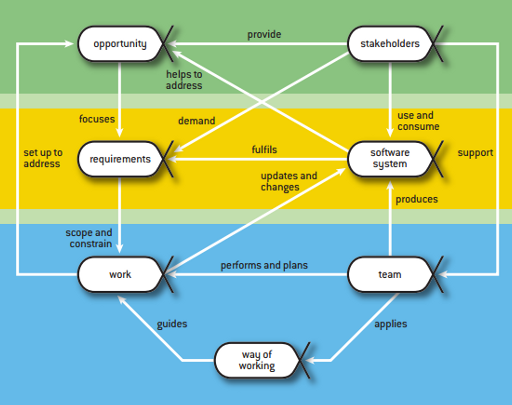
\includegraphics[height=9cm]{alpha-semat}
		\caption{Rappresentazione, di alto livello, dei legami 
			     sussistenti tra differenti concetti alpha. Immagine tratta 
				 da: http://bit.ly/2g5oV7b.}
	\end{center}
\end{figure}  

\newpage 

La \textbf{Figura 3.1} presenta l'insieme degli alpha e le relazioni 
sussistenti tra gli alpha adiacenti, su proposta di Ivar Jacobson, 
il pioniere dell'iniziativa SEMAT. 
 
I colori, invece, rappresentano le aree di competenza per la valutazione 
dello stato del progetto. Ciascun colore corrisponde a un obiettivo finale; 
questi obiettivi sono: 

\begin{itemize}
	\item Livello di fidelizzazione del cliente - colore verde;
	\item Maturità della soluzione e della rispettiva implementazione - colore giallo;
	\item Il \textit{backlog} di lavoro - colore blue.
\end{itemize}

Un'interpretazione simile della realtà offre una maggior 
tracciabilità dello stato di avanzamento del progetto. 
Per esempio, in \textbf{Figura 3.2}, l'alpha dei requisiti  
offre un ottimo spunto di riflessione sulla maturità e 
stabilità dei requisiti, individuati nella fase di AdR 
(Analisi dei Requisiti). 
Inoltre, esiste per ciascun alpha un insieme di indicatori, 
che guidano, rispetto al piano iniziale di lavoro, l'andamento 
e la qualità del lavoro complessivo. 
Tramite una lista di controllo, SEMAT propone un modo indipendente 
da processi aziendali di valutazione 
del completamento degli obiettivi.

\begin{figure}[htbp]
	\begin{center}
		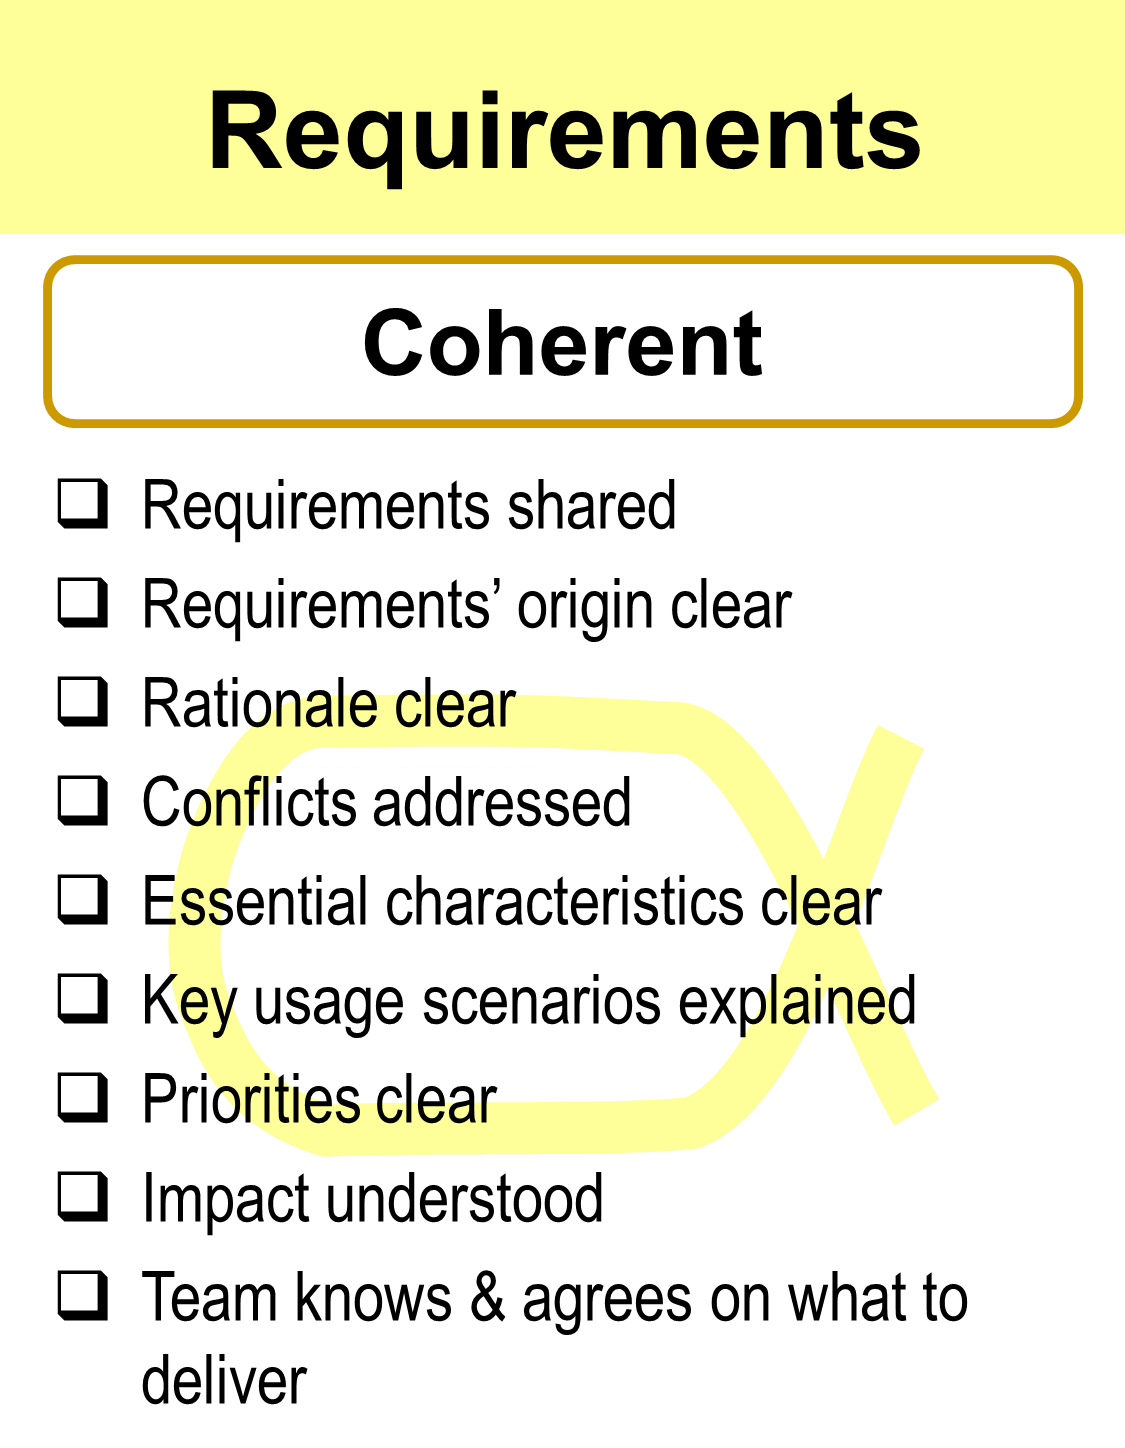
\includegraphics[height=6cm]{requirements-semat}
		\caption{Ogni concetto alpha è caratterizzato da un 
			     insieme di elementi descrittivi, come: nome, 
			     l'obiettivo e la lista di controllo. Immagine tratta 
				 da: http://bit.ly/2vgPqJf.}
	\end{center}
\end{figure}  

La rappresentazione dei temi frequenti in un progetto 
software tramite gli alpha incrementa la comprensione
generale del gruppo di lavoro.

Per esempio, il alpha dei requisiti è caratterizzato 
dal seguente insieme di obiettivi da raggiungere:

\begin{itemize}
	\item \textit{Conceived}: Dimostrata necessità per un nuovo prodotto;
	\item \textit{Bounded}: Lo scopo del nuovo prodotto sono chiari;
	\item \textit{Coherent}: I requisiti offrono una chiara prospettiva del nuovo prodotto software;
	\item \textit{Acceptable}: I requisiti descrivono il prodotto che è accettato dal cliente;
	\item \textit{Addressed}: Una buona parte dei requisiti sono stati implementati, il sistema 
	      soddisfa la visione che il cliente ha del sistema;
	\item \textit{Fulfilled}: I requisiti che sono stati affrontati sono in accordo con gli 
	      obiettivi pattuiti con il cliente.
\end{itemize} 

Durante l'analisi dei requisiti, ho utilizzato questi obiettivi per valutare
lo stato del mio lavoro, rispetto alla pianificazione iniziale. 
Inoltre, quando ho raggiunto l'obiettivo \textit{"Coherent"} dei requisiti,
ho acquisito una buona visione del sistema da sviluppare nel complesso    
Infatti, la lista di controllo, in allegato a ciascun alpha, mi ha guidato  
nell'attività di consuntivazione. Ho trovato d'aiuto questa lista 
di controllo anche come fonte di requisiti e domande critiche
sul progetto e sistema.   

Ho utilizzato, per esempio, questa griglia per valutare la mia situazione
di progresso rispetto alla pianificazione di periodo. 

%\newpage 

Per un maggior controllo e visibilità del grado di 
completamento del progetto, ho utilizzato l'applicazione "SematAcc", 
che è raggiungibile al seguente indirizzo 
\url{http://sematacc.herokuapp.com/}. 
L'applicazione mi ha permesso, grazie al cruscotto intuitivo 
da essa offerto, di concentrare la mia attenzione su obiettivi di valore 
aggiunto al progetto e temporeggiare con le attività di priorità
più bassa. In questo modo, ho ottenuto un modo agile e semplice 
per gestire i rischi.

A progetto concluso, la situazione del progetto è come in
\textit{Figura 3.3}. I dati, che presento, mostrano uno stato 
salutare per il progetto. Questi dati non rappresentano il massimo
valore; visto che, gli obiettivi sono in continua evoluzione, come 
le tecnologie. 

Ho pianificato e trattato il margine 
rimanente come un margine di evoluzione 
e miglioramento del sistema.

\begin{figure}[htbp]
	\begin{center}
		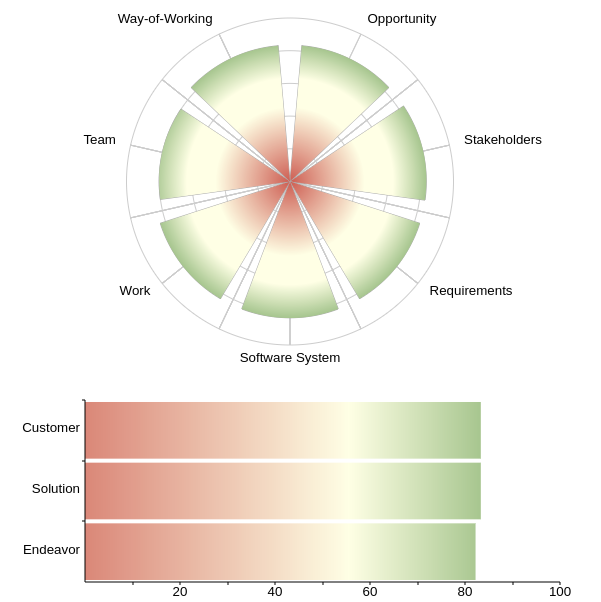
\includegraphics[height=8cm]{final-semat}
		\caption{Rappresentazione dello stato del progetto, 
			a seguito dell'ultima consegna ufficiale e 
			superamento della revisione di accettazione.}
	\end{center}
\end{figure}  

Aderire all'iniziativa SEMAT e seguire approcci metodologici  
flessibili è vantaggioso. Nel mio caso, ho composto un proprio 
metodo di lavoro; ho ottenuto una semplice gestione dei 
rischi e ho migliorato la mia sensibilità per recepire 
lo stato del progetto in modo naturale ed intuitivo. 
Inoltre, ho migliorato la metodologia di lavoro e, 
con disciplina, ho acquisito le capacità di controllo 
sull'incertezza, in momenti di decisioni importanti. 

%\newpage 

\section{Pianificazione}
Durante lo stage ho lavorato 316 ore. 
Complessivamente, queste ore corrispondono poco 
più di 8 settimane di lavoro effettivo. Nel mio 
caso, lo stage è iniziato il 12/12/2016 e 
terminato il 20/02/2017. In questo arco di 
tempo, è incluso anche il periodo delle 
festività natalizie. Causa assenze impreviste 
da parte mia, nell'ultima settimana di lavoro,
ho esteso la terminazione dello stage dal 
giorno 20/02/2017 al 23/02/2017.

\begin{figure}[htbp]
	\begin{center}
		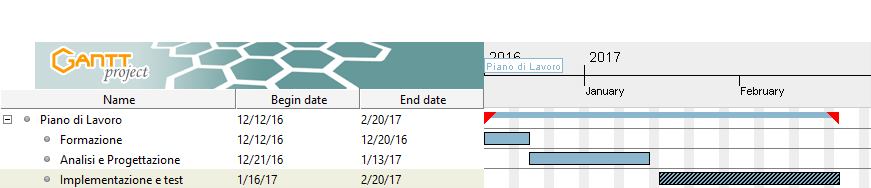
\includegraphics[height=3cm]{piano-di-lavoro}
		\caption{Piano di lavoro ufficiale.}
	\end{center}
\end{figure}

In \textbf{Figura 3.4} presento il diagramma di Gantt del piano 
di lavoro,  i cui dettagli ho descritto
\hyperref[sec:piano-di-lavoro]{sezione Piano di Lavoro}.  

Il diagramma di Gantt presenta una pianificazione generica del PdL; 
tuttavia, essendo io libero nell'organizzazione del lavoro, 
ho rivisto e riprogrammato le attività del PdL come in \textbf{Figura 3.5}. 

\begin{figure}[htbp]
	\begin{center}
		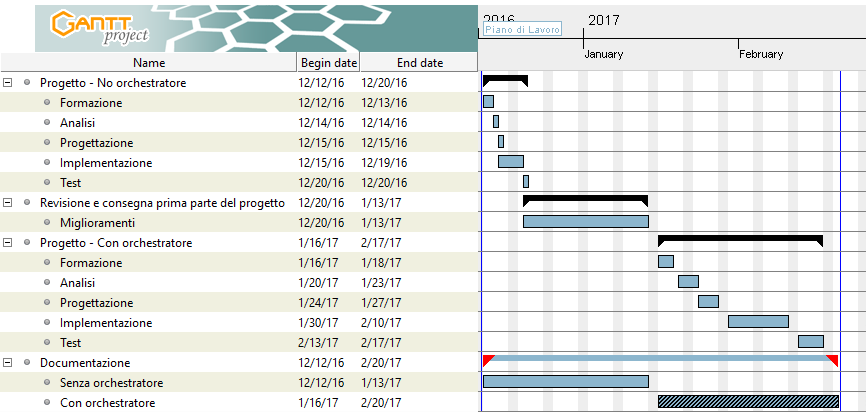
\includegraphics[height=6cm]{piano-lavoro-dettaglio}
		\caption{Piano di lavoro rivisto e riorganizzato.}
	\end{center}
\end{figure} 

Il progetto prevede la containerizzazione di una soluzione di
"\textit{Malware Dashboard}" e il rilascio del sistema containerizzato
in un ambiente con e senza orchestratore. In relazione con le modalità 
richieste di messa in esercizio del sistema, ho 
organizzato il lavoro complessivo in due mini progetti.
Ho orientato il primo progetto al rilascio del sistema in un contesto 
containerizzato senza orchestratore, qui ho utilizzato unicamente la 
tecnologia Docker, e un secondo progetto orientato 
all'orchestrazione di container, qui ho utilizzato la tecnologia Kubernetes.
Il secondo progetto ha esteso il primo da un punto di visto 
di un incremento migliorativo.

Come parte di riuso tra i due progetti, ho utilizzato 
l'architettura del sistema complessivo e le componenti 
containerizzate. Una simile organizzazione del progetto 
di stage, mi ha permesso di pianificare i momenti di  
\textit{sprint}; uno sprint è un insieme di compiti, 
usualmente, di breve durata e molto intensi di lavoro. Ho scelto
di operare in questo modo perché ho ritenuto importanti i \textit{feedback} 
del tutor aziendale. Inoltre, ho utilizzato questi feedback come una metrica di 
avanzamento, raggiungimento degli obiettivi e maturità della soluzione. Inoltre, 
conoscere il punto di vista del tutor ha garantito stabilità alla soluzione 
per l'implementazione del sistema. 

\section{Attività di formazione}

Ho seguito un metodo attivo di formazione. Ho arricchito le 
attività di studio teorico con attività di laboratorio. 
Durante le sessioni pratiche, ho svolto piccoli 
progetti. Tramite questi piccoli progetti, ho toccato 
con le mani le tecnologie alla base dello stage. 

\subsection{Docker}

Ho imparato la tecnologia, Docker, allo stato dell'arte della 
containerizzazione. Durante la formazione su Docker, ho 
appreso i concetti alla base della tecnologia, come utilizzare 
lo strumento e come pensare i sistemi orientati ai container.

Tramite il frammento di codice, che allego in seguito, illustro 
come estendere un'immagine Docker della componente d'esempio 
Elasticsearch con una estensione di terzi parti; 
questo frammento di codice è chiamato Dockerfile.

\begin{verbatim}
FROM elasticsearch:2.4
MAINTAINER Andrei Petrov <apetrov.ya@yandex.ru>
ADD hq.tar /usr/share/elasticsearch/plugins
\end{verbatim}

Il Dockerfile rappresenta la configurazione 
di componente e le sue dipendenze software. 
In un altro modo, il Dockerfile descrive 
in modo dichiarativo le dipendenze esterne 
del processo. Il Dockerfile è necessario per 
la creazione dell'immagine. Dall'immagine, invece, 
si possono istanziare, possibilmente, infiniti processi. 
Inoltre, un'informazione curiosa sulla chiave \textbf{ADD}
è la seguente: la direttiva permette, in modo automatico,
l'estrazione di file da un archivio con estensione tar.
Questo \textit{hack} è utilissimo e molto amato
dagli esperti di containerizzazione Docker. 
La direttiva è uno \textit{shortcut} che 
permette di ridurre a una sola registrazione sul 
\textit{Augmented File System}, utilizzato da Docker
per la memorizzazione della configurazione dei container. 
Altrimenti, per copiare un archivio da un contesto 
all'altro durante la creazione dell'immagine, devo
copiare l'archivio e successivamente estrarre i dati.
Anche io preferisco utilizzare la direttiva "ADD".

Quando un prodotto software complesso è costituito da 
un insieme di componenti containerizzate, un modello 
mentale utile per la comprensione delle relazioni tra 
le immagini Docker è il modello ad ereditarietà singola 
dei linguaggi di programmazione ad oggetti, come per
esempio il linguaggio di programmazione Java.
Le immagini, come in alcuni casi le classi, 
possono essere organizzate tramite estensioni.
Questo modello favorisce il riciclo delle 
componenti.

Ho utilizzato i Dockerfile come template 
per la creazione di immagini e container di servizi. 
Questo approccio mi ha permesso di codificare in un file, 
da un lato, un insieme di configurazioni parametrizzate;
dall'altro, includere fisicamente nel package
le dipendenze esterne. In seguito alla codifica dei Dockerfile
ho notato un notevole incremento della mia produttività.

La tecnologia Docker ha rivoluzionato il mondo dello 
sviluppo del software. Questa tecnologia ha introdotto 
uno standard per il confezionamento del software.

Un esempio di istanziazione di un container applicativo
Elasticsearch è il seguente:
 
\begin{verbatim}
docker run -d \
-p $(ES_MASTER_CONTAINER_HTTP_PORT):$(ES_MASTER_CONTAINER_HTTP_PORT) \
-p $(ES_MASTER_CONTAINER_TCP_PORT):$(ES_MASTER_CONTAINER_TCP_PORT) \
--name $(MASTER_CONTAINER_NAME) \
--volumes-from $(ES_DATA_CONTAINER_NAME) \
-v limits.conf:/etc/security/limits.conf \
$(ES_DOCKER_IMG):$(ES_DOCKER_IMG_VERSION) \
-Des.node.name="$(MASTER_ES_NODE)" \
-Des.cluster.name="$(ES_CLUSTER_NAME)" \
-Des.node.master="true" \
-Des.node.data="false"  \
-Des.index.number_of_shards=$(ES_SHARDS_NUM) \
-Des.index.number_of_replicas=$(ES_REPLICAS_NUM) \
-Des.network.host=_site_ \
...
-Des.gateway.recover_after_nodes=2 \
-Des.gateway.expected_nodes=2 \
...		 
\end{verbatim}

Qui, tramite la CLI (Command Line Interface) di Docker, creo e 
ed eseguo un container in modalità demone (processo eseguito in background). 
Successivamente, configuro le porte logiche per abilitare la 
comunicazione interprocesso via rete; specifico un \textit{bucket} 
logico per la condivisione dei dati tra il server e il container, 
tramite le opzioni "--volumes-from" e "-v";  fornisco un alias 
mnemonico al container, tramite l'opzione "--name" ed ecc.
Le opzioni con il prefisso "-Des" rappresentano le configurazioni 
per il processo Java di Elasticsearch. In questo frammento di codice
ho omesso alcune parti.
 
Per verificare le mie conoscenze preliminari su container e Docker, 
ho implementato uno script Bash con l'obiettivo di creare un 
cluster di \texttt{N} nodi di Elasticsearch 
in modo automatico ed autonomo.  Il cluster creato è rilasciato 
in modalità locale alla macchina virtuale ospitante.
Su un insieme di \texttt{N} nodi, \texttt{N - M} nodi sono di 
tipologia "data" e il resto sono di tipologia "master". 
Il numero minimo di nodi master è dato dalla 
seguente formula \texttt{M\_min = M/2 + 1}. 
La quantità \texttt{M\_min} specifica il \textit{quorum} 
iniziale di nodi, necessario per la procedura di elezione 
di un nuovo leader del cluster. 

\subsection{Kubernetes}

L'orchestratore è indispensabile per una efficiente gestione 
di una flotta di container. Durante il periodo di formazione, 
ho affrontato diversi problemi legati al presente orchestratore. 
Alcuni di questi problemi riguardano la creazione di un cluster 
Kubernetes in configurazione semplice. Questa configurazione 
interessa la creazione di un cluster formato da nodi master 
e worker. La configurazione del cluster è sprovvista di alta affidabilità. 
Ho effettuato questa scelta causa la difficoltà della procedura 
di installazione e configurazione di un cluster Kubernetes 
in alta affidabilità. Un cluster Kubernetes può essere creato 
tramite strumenti di terzi parti della tecnologia, fornite
come moduli esterni che estendono il prodotto base. 
Un simile strumento, per esempio, è \textbf{kubeadm}. Inoltre, è 
possibile creare un cluster Kubernetes a mano. Quest'ultima modalità 
è macchinosa e lunga. Durante lo stage ho favorito 
la semplicità; con lo strumento \textit{kubeadm} ho effettuato 
il \textit{deployment} di un cluster Kubernetes in 
breve tempo. Lo strumento gestisce in modo
automatico tutti i passi di configurazione iniziale. 
Inoltre, \textit{kubeadm} offre una procedura di distruzione del
cluster.

Ad esempio, tramite il semplice comando 
\begin{verbatim}
kubeadm init
\end{verbatim}
ho installato e configurato un nodo master di Kubernetes. 
Successivamente, con il token generato, ho aggiunto ulteriori 
nodi worker al nodo master esistente. Per aggiungere un nuovo 
nodo worker ho usato, invece, il seguente comando: 
\begin{verbatim}
kubeadm join <token> <indirizzo IP del master>
\end{verbatim}

Durante l'attività di formazione su Kubernetes ho svolto 
attività di studio mirate all'amministrazione dell'infrastruttura 
Kubernetes e all'organizzazione delle risorse containerizzate 
tramite gli oggetti nativi dell'orchestratore, per esempio: 
ReplicationController, Services, Deployments, Job ed ecc., 
affinché l'orchestratore possa gestire i container in esecuzione. 
L'oggetto base di Kubernetes è il Pod. Questa risorsa è una capsula dove al centro  
risiede un container Docker. Un Pod è anche l'unita atomica di schedulazione.

Per la codifica degli oggetti di Kubernetes ho utilizzato dei file.
Questi file sono un modo dichiarativo per codificare l'infrastruttura.
Nella comunità di Kubernetes essi vengono chiamati \textit{manifest}. 

Un esempio di manifest, che ho codificato, è il seguente

\begin{verbatim}
---
apiVersion: v1
kind: Service
metadata:
namespace: elk-dev
name: elasticsearch
labels:
  component: elasticsearch
  role: client
spec:
 selector:
 component: elasticsearch
 role: client
 ports:
 - name: http
   port: 9200
   protocol: TCP
---
apiVersion: v1
kind: ReplicationController
metadata:
  name: es-client
  namespace: elk-dev
  labels:
   component: elasticsearch
   role: client
spec:
 replicas: 1
 ...

\end{verbatim}

Il linguaggio che ho utilizzato per la 
stesura dei manifest di Kubernetes è il linguaggio 
di markup YAML (Yet Another Markup Language). I manifest 
possono essere stesi in due formati: JSON e YAML. Ho utilizzato
il secondo per facilitare la lettura. Il manifest 
allegato è un esempio parziale di 
configurazione in codice di una componente Elasticsearch 
dell'infrastruttura. La prima risorsa è un Service. 
Un Service implementa la funzionalità di \textit{Service Discovery}. 
Infatti, i microservizi utilizzano i nomi dei Service per abilitare
la comunicazione. La seconda risorsa, invece, rappresenta un 
ReplicationController. Il ReplicationController dichiara che il 
numero di copie per lo specifico microservizio deve essere sempre 
pari a uno; lo stato di questa risorsa è gestito dalla componente 
controller di Kubernetes. In caso che, lo stato della
risorsa inizierà a divergere , il controller riporterà allo stato
specificato la risorsa. Questa funzionalità permette, in caso di errore, 
di schedulare nuovamente il Pod e risanare lo stato della componente tramite 
una sequenza di riavvi continui. E in questo caso il controller 
di Kubernetes segnalerà il motivo di errore della risorsa. Questa funzionalità 
si chiama \textit{self-healing}. 
I dati dei pod possono essere salvati su volumi di memorizzazione esterni. 

La specifica di qualsiasi risorsa è costituita 
da quattro parti fondamentali: apiVersion, kind, template e spec. 
La chiave "apiVersion" determina la versione delle API di Kubernetes 
da utilizzare quando dobbiamo specificare una risorsa di tipo "kind".
Ogni chiave-valore presente internamente alla sezione template deve 
essere interpretata come una meta informazione necessaria all'amministrazione 
delle risorse. Infine, il contesto "spec" descrive la specifica per la risorsa.
Le specifiche riguardano la codifica dello stato della risorsa.

La tecnologia Kubernetes offre una macchina a stati per la gestione dei container.
Questo modello a stati, introdotto da Kubernetes, permette diversi problemi 
legati alla qualità dei servizi, alla quantità di risorse 
utilizzate da ciascuna risorsa ed ecc.

\subsection{Clustering di Elasticsearch}
Una delle caratteristiche più importanti di Elasticsearch è
la funzionalità di \textit{clustering}. Questa funzionalità
permette di eseguire in parallelo un insieme di 
processi Elasticsearch sotto uno spazio di nomi
comune. La singola componente, di un cluster, prende 
il nome di nodo. I nodi di un cluster condividono
dati. L'organizzazione dei dati e la politica della 
loro gestione, in modalità cluster,
è complessa. Durante il periodo di formazione 
ho appreso come creare, organizzare i dati e gestire
la componente Elasticsearch in modalità \textit{clustering}.

Approfondito il concetto di clustering in Elasticsearch,
ho implementato degli script per automatizzare e velocizzare
le procedure di manutenzione del cluster Elasticsearch. 

Se da un lato, il clustering incrementa la percentuale di 
\textit{High Availability}, da un altro lato è necessario 
analizzare i requisiti d'uso del cluster. L'analisi d'uso 
è necessaria per comprendere come configurare i livelli di 
ridondanza dei dati e l'organizzazione di partizionamento
degli indici gestiti da Elasticsearch. Nella terminologia 
Elasticsearch un indice è un database. Durante la formazione
su Elasticsearch, ho realizzato che esigenze di scrittura 
possono impattare le performance del cluster se il 
numero delle repliche è elevato. Questo fenomeno è
dovuto alla grande latenza di propagazione delle 
scritture su ciascuna copia dei dati memorizzati.
Al contrario, in caso di esigenze di lettura, ho 
notato che un alto numero di repliche 
migliora di molto i tempi di risposta del cluster 
Elasticsearch.  

\section{Analisi dell'alta affidabilità}
Una delle più importanti garanzie che il settore IT deve garantire 
al business è la continuità operativa dei servizi informatici a 
supporto. I servizi informatici sono complessi e distribuiti.
A causa della loro natura distribuita, i sistemi informatici 
possono essere sottoposti a problemi, per esempio, di rete, 
che degradano la qualità di erogazione di questi servizi.

L'alta affidabilità è un'abilità, del sistema, che permette
di  garantire la continuità operativa, anche se le singole 
componenti non sono in uno stato di buona salute. L'analisi 
dell'alta affidabilità ha l'obiettivo di comprendere 
a fondo i dettagli della proprietà di alta affidabilità
dell'intero sistema da realizzare. 

In questa fase ho individuato due livelli esclusivi che interessano
l'alta affidabilità: un livello fisico/virtualizzato e uno 
logico/containerizzato. Su raccomandazione del mio tutor aziendale, 
ho tralasciato lo studio dell'alta affidabilità 
a livello fisico e mi sono concentrato su quello logico.
A questo livello, ho analizzato quali sono le componenti 
che possono mettere a rischio lo stato complessivo del sistema.

Nella tabella a seguire, riporto le tecnologie utilizzate e per ciascuna 
di esse caratterizzo la tipologia di applicazione e il rispettivo livello 
di supporto per il clustering.

\begin{center}
\begin{tabular}
	{l||p{5cm}||p{5cm}}	
	\arrayrulecolor{white}
	\rowcolor{glaucous}	
	Componente 	&  
	\makebox[4cm][c]{Tipologia} & 	
	\makebox[5cm][c]{Supporto nativo clustering} \\ 
	\rowcolor{lightcornflowerblue}
	Elasticsearch & 
	\makebox[4cm][c]{Applicazione Java} & 
	\makebox[5cm][c]{Si} \\
	\rowcolor{moonstoneblue}
	Kibana & 
	\makebox[4cm][c]{Applicazione Javascript} & 
	\makebox[5cm][c]{No} \\
	\rowcolor{lightcornflowerblue}
	Logstash & 
	\makebox[4cm][c]{Applicazione Java} & 
	\makebox[5cm][c]{No} \\
	\rowcolor{moonstoneblue}
	Nginx & 
	\makebox[4cm][c]{Applicazione C++} & 
	\makebox[5cm][c]{Si} \\
\end{tabular}		  
\end{center}
\captionof{table}{Elenco delle tecnologie utilizzate con il supporto nativo per il clustering} 

Dalla tabella segue che, alcune componenti non 
offrono un supporto nativo per il clustering.
Per garantire la continuità di servizio, ho 
utilizzato il concetto di \textit{redundancy}. 
Tramite l'esecuzione parallela di più 
processi dello stesso tipo, posso garantire
la continuità di erogazione del servizio, anche 
se al più tutti meno uno di questi processi
,all'improvviso, falliscono. Ad alto livello, 
l'utente può, eventualmente, risentire un 
degrado di \textit{performance}. 
Un ulteriore elemento della mia analisi è stata 
la garanzia del basso accoppiamento 
tra le componenti del sistema. 

Come strumento a supporto dell'analisi dell'alta affidabilità, 
ho utilizzato il modello a cubo della scalabilità. 
Il modello offre tre dimensioni X,Y e Z. Ciascuna dimensione 
rappresenta una oggetto di studio. Per esempio, Elasticsearch
è un'applicazione distribuita che offre nativamente 
il supporto per la scalabilità orizzontale e il partizionamento 
dei dati. Una conseguenza importante da notare in Elasticsearch
è il livello della consistenza. Infatti, Elasticsearch è un 
database NoSQL e non garantisce l'alta consistenza. Questo
è il prezzo da pagare quando l'obiettivo del sistema è la scalabilità
su larga scala.

Sebbene la scalabilità implica l'alta affidabilità, 
per esempio tramite la ridondanza, ho ritenuto 
il modello della scalabilità a cubo un concetto 
importante per comprendere le dimensioni 
dell'alta affidabilità del sistema.

\begin{figure}[htbp]
	\begin{center}
		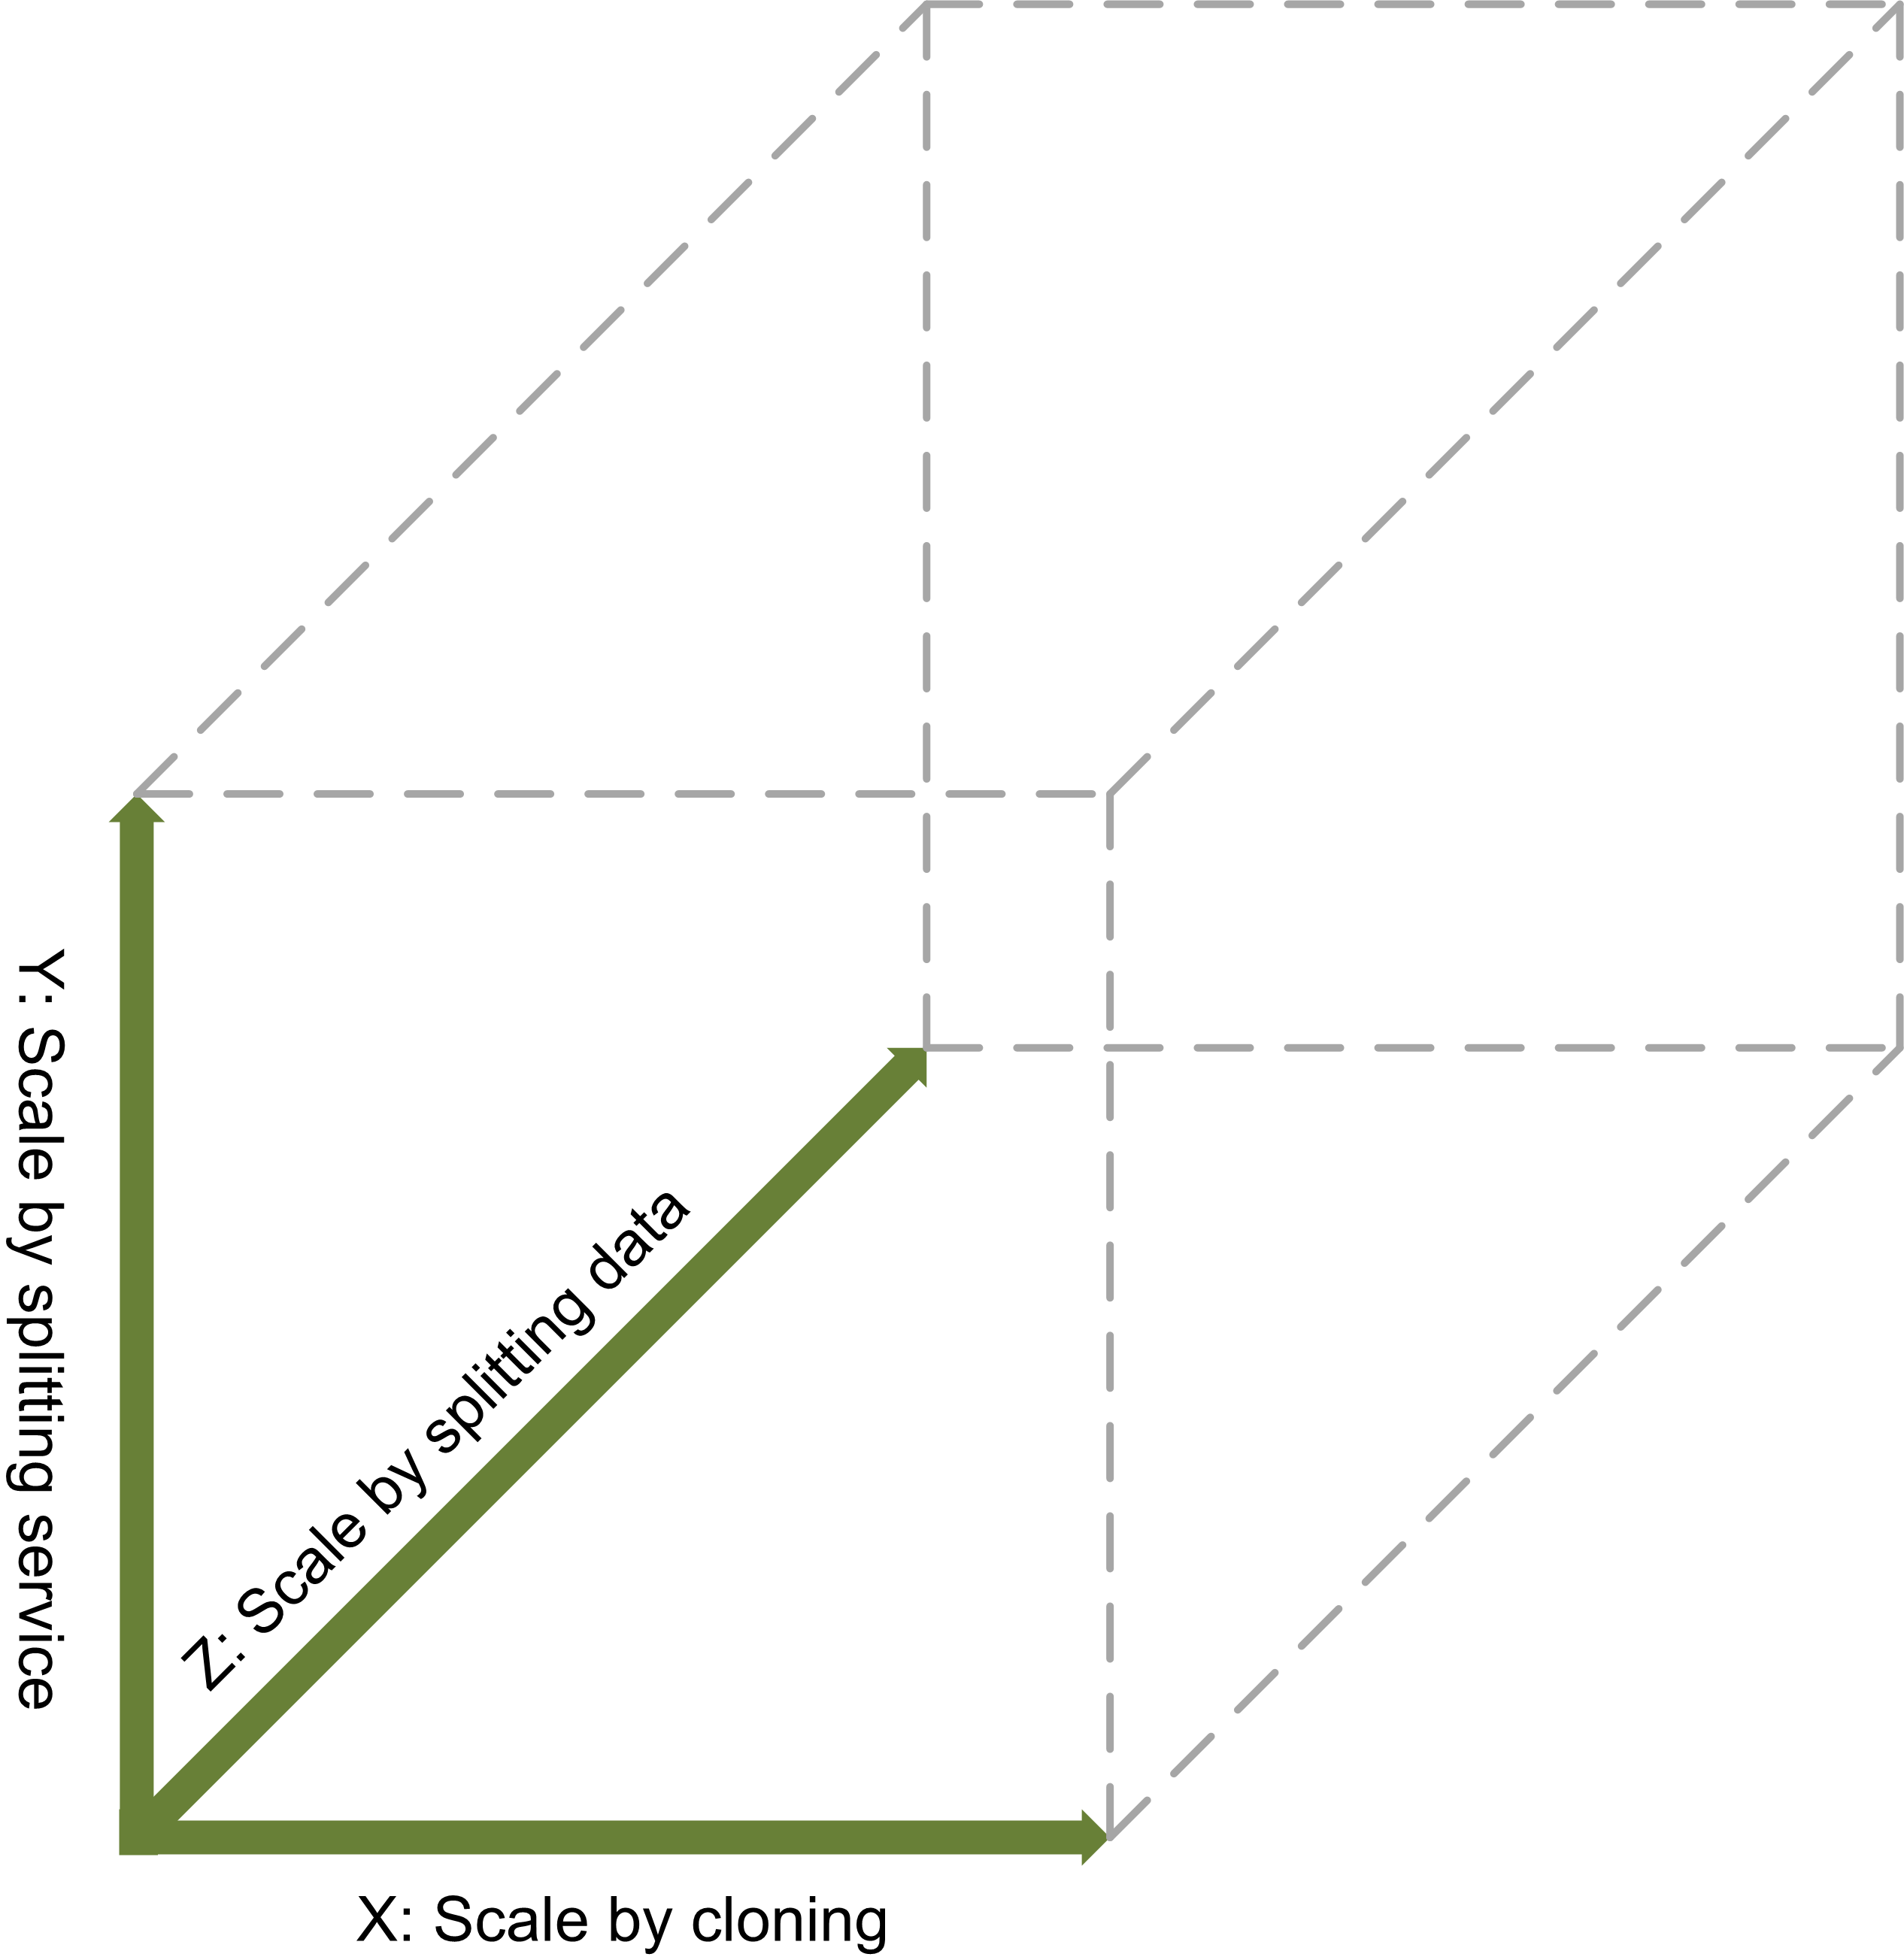
\includegraphics[height=6cm]{scale-cube}
		\caption{Interpretazione grafica del modello a cubo della scalabilità.
		        Immagine tratta da: http://bit.ly/2wPA42R}
	\end{center}
\end{figure}

La dimensione del sistema determina la difficoltà di gestione. 
La difficoltà di gestione incrementa la probabilità
che a regime (sistema operante a tempo pieno) il sistema
possa rivelare un comportamento non atteso. La garanzia di un appropriato
livello di servizio favorisce un accordo equo tra il fornitore del
servizio e l'utilizzatore. Una metrica che ho 
fissato per la qualità di erogazione del servizio è la classe 3 
di alta affidabilità. Ho calcolato questa metrica tramite 
i test di carico e i test di durata. 

La possibilità di valutare a regime la qualità del servizio 
è un obiettivo dei prossimi incrementi evolutivi del progetto. 
Al momento dello stage ho ritenuto questo obiettivo un requisito opzionale.

Per la misura dell'alta affidabilità,
ho utilizzato la seguente scala espressa in tabella.

\begin{center}
\begin{tabular}
		{l||p{5cm}||p{2cm}||p{2cm}}	
		\arrayrulecolor{white}
		\rowcolor{glaucous}	
		Tipo di sistema &  
		\makebox[5cm][c]{Disservizio (minuti per anno) } & 	
		\makebox[2cm][c]{Affidabilità} & 
		\makebox[2cm][c]{Classe} \\ 
		\rowcolor{lightcornflowerblue}
		Non gestito & 
		\makebox[5cm][c]{50000} & 
		\makebox[2cm][c]{90}  & 
		\makebox[2cm][c]{1} \\
		\rowcolor{moonstoneblue}
		Gestito & 
		\makebox[5cm][c]{5000} & 
		\makebox[2cm][c]{99} & 
		\makebox[2cm][c]{2} \\
		\rowcolor{lightcornflowerblue}
		Bene gestito & 
		\makebox[5cm][c]{500} & 
		\makebox[2cm][c]{99.9} & 
		\makebox[2cm][c]{3} \\
		\rowcolor{moonstoneblue}
		Tollerante ai guasti & 
		\makebox[5cm][c]{50} & 
		\makebox[2cm][c]{99.99} & 
		\makebox[2cm][c]{4} \\
		\rowcolor{lightcornflowerblue}
		Altamente affidabile & 
		\makebox[5cm][c]{5} & 
		\makebox[2cm][c]{99.999} & 
		\makebox[2cm][c]{5} \\
\end{tabular}		  
\end{center}
\captionof{table}{Categorizzazione delle classi di affidabilità dei sistemi informatici. Materiale tratto da: http://bit.ly/2wlGrbn.} 

L'incremento della classe di alta affidabilità è 
un'attività  che richiede costanza e automazione.
I sistemi caratterizzati da alte classi di alta
affidabilità richiedono che essi vengano progettati 
per essere il più possibile autonomi.

\section{Progettazione ed implementazione}
Con la presente sezione descrivo l'architettura di alto
livello del sistema.

\subsection{Vista architetturale}
Per la modellazione di alto livello del sistema ho utilizzato 
lo stile architetturale a Microservizi. Questo stile promuove
la dimensione Y del modello a cubo della scalabilità. Infatti, 
lo stile architetturale a Microservizi porta all'estremo 
il concetto del partizionamento delle funzionalità.
In questo contesto, una funzionalità individua un processo.
Con l'ausilio dei container i microservizi vengono containerizzati.
Per ottenere la scalabilità orizzontalmente è sufficiente aggiungere un nuovo 
processo, copia del processo containerizzato in esecuzione e 
bilanciare il traffico verso l'insieme di processi cosi ottenuto.

In figura che segue, presento i microservizi costituenti il sistema 
da me realizzato.
\newpage
\begin{figure}[htbp]
	\begin{center}
		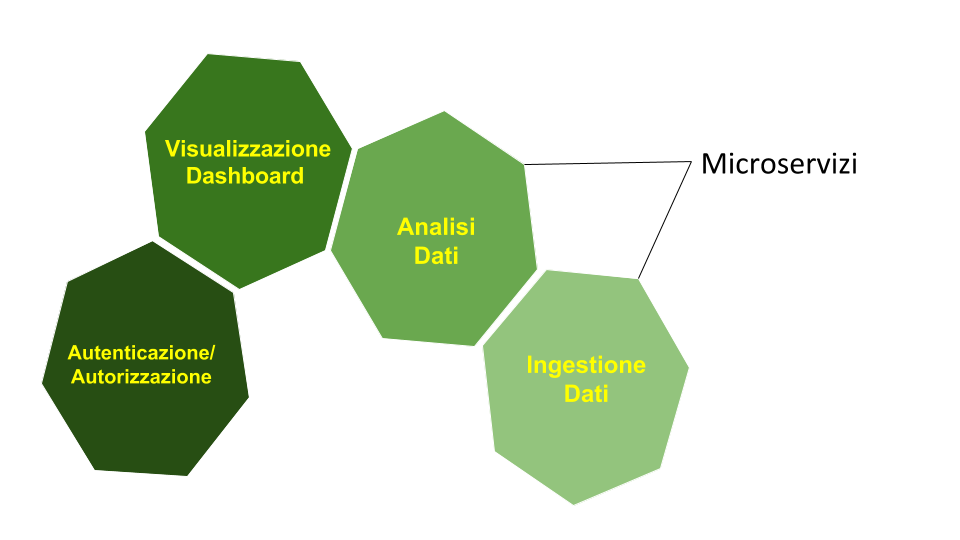
\includegraphics[height=6cm]{microservizi}
		\caption{Visione di alto livello dell'architettura del sistema.}
	\end{center}
\end{figure}  

Ogni microservizio è responsabile di una sola funzionalità. 
Le figure esagonali sono una convenzione diffusa per 
rappresentare i singoli microservizi costituenti 
un'architettura a Microservizi. Questa notazione ha origine 
nel pattern architetturale "Hexagon Design Pattern", 
promosso da Alistair Cockburn.

%\newpage 

In tabella, per ogni microservizio riporto
una breve descrizione della funzionalità e la tecnologia 
utilizzata per la sua implementazione.  

\begin{center}
	\begin{tabular}
		{l||p{5cm}||p{4cm}}	
		\arrayrulecolor{white}
		\rowcolor{glaucous}	
		Microservizio &  
		\makebox[5cm][c]{Funzionalità) } & 	
		\makebox[4cm][c]{Tecnologia} \\
		\rowcolor{lightcornflowerblue}
		Autorizzazione/Autenticazione & 
		\makebox[5cm][c]{Gestione degli accessi} & 
		\makebox[4cm][c]{Nginx}  \\
		\rowcolor{moonstoneblue}
		Visualizzazione & 
		\makebox[5cm][c]{Gestione delle dashboard} & 
		\makebox[4cm][c]{Kibana} \\
		\rowcolor{lightcornflowerblue}
		Analisi dati & 
		\makebox[5cm][c]{Gestione dei dati in analisi} & 
		\makebox[4cm][c]{Elasticsearch} \\
		\rowcolor{moonstoneblue}
		\textit{Ingesting} & 
		\makebox[5cm][c]{Raccolta ed inserimento dei dati} & 
		\makebox[4cm][c]{Logstash} \\ 
		\rowcolor{lightcornflowerblue}
	\end{tabular}		  
\end{center}
\captionof{table}{Elenco dei microservizi costituenti il sistema.}
%\newpage

\subsection{Flusso operativo}
Il sistema che ho progettato è caratterizzato da un alto tasso di coesione e 
basso accoppiamento. In figura a seguire, con l'ausilio dell'indicazione
numerica, presento i flussi di dati che il sistema deve gestire.

\begin{figure}[htbp]
	\begin{center}
		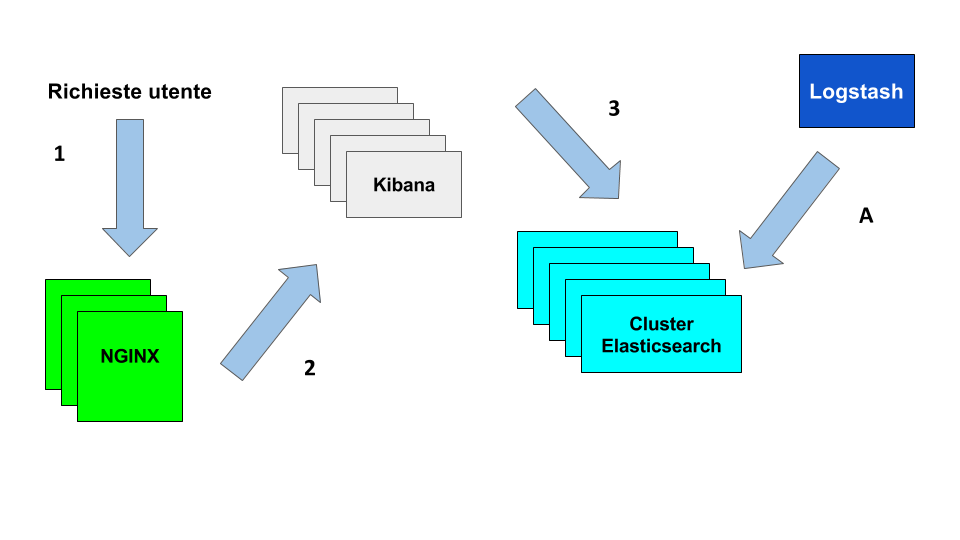
\includegraphics[height=6.5cm]{flusso}
		\caption{Indicazione dei flussi di dati e delle dipendenze dei microservizi.}
	\end{center}
\end{figure} 

\newpage 

Il sistema è caratterizzato da due flussi distinti.

\begin{enumerate}
	\item \textbf{Flusso 1-2-3}:  \\
	Il seguente flusso rappresenta il flusso inerente
	alla parte esposta all'uso degli utenti.
	\begin{figure}[htbp]
		\begin{center}
			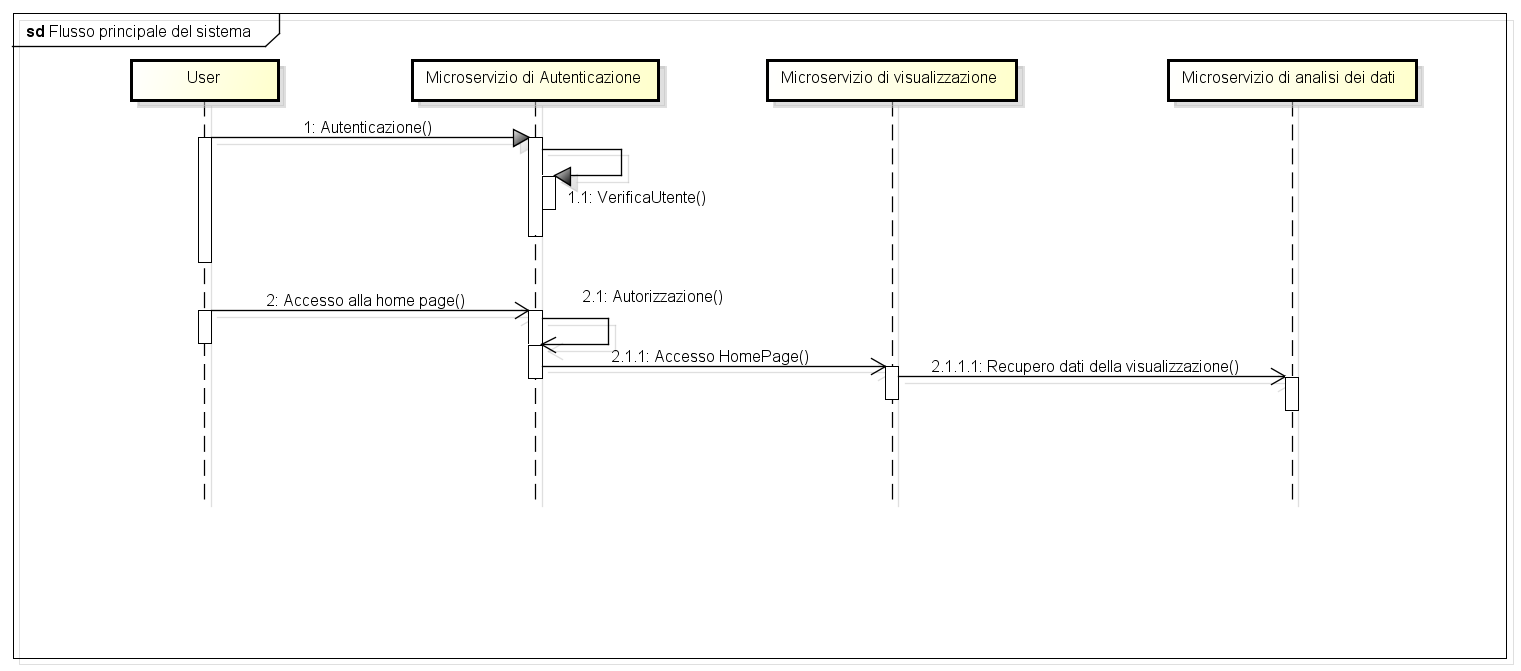
\includegraphics[height=6.5cm]{flusso-principale}
			\caption{Descrizione di alto livello dell'interazione dell'utente con il sistema.}
		\end{center}
	\end{figure} 
    \newpage  
	\item \textbf{Flusso A}: \\
	Un'ulteriore flusso interessa il processo di raccolta ed inserimento dei dati
	nel sistema. Lo strumento ETL (Extract Transform and Load) utilizzato è Logstash.
	Questo flusso non impatta le perfomance complessive del sistema, in quanto 
	la sorgente dati è statica, ha una dimensione fissa. Il flusso è operativo
	solo durante la prima installazione del cluster, successivamente esso 
	è disattivato.
\end{enumerate}

\subsection{Organizzazione del cluster Elasticsearch}

Dal punto di vista applicativo e in contesto WEB, Elasticsearch
può essere interpretato come un backend, ovvero una sorgente di dati. 
Questa componente supporta diverse configurazioni topologiche
di nodi. L'insieme di nodi che non ho trattato sono i nodi per 
la comunicazione inter cluster e distribuiti su zone geografiche diverse.
Un \textit{use case} comune per l'utilizzo di questo tipo di nodi è 
la replica dei dati tra due \textit{Data Center} diversi. 

La progettazione del cluster che ho trattato riguarda una configurazione
di nodi distribuiti nella stessa zona geografica.

In contesto con orchestratore Kubernetes, il cluster minimale è composto 
dal seguente insieme: 1 nodo data, 1 nodo master e 1 nodo client. 
L'ultimo nodo ha il compito di bilanciare il traffico esterno proveniente 
dagli utenti connessi al cluster. Inoltre, i nodi di tipo client mantengono 
una tabella informativa su quale nodo mantiene uno specifico 
frammento di dato. Ho progettato in questo modo l'architettura del sistema 
per agevolare la scalabilità orizzontale delle componenti. Un vincolo forte
per la scalabilità dei nodi master è il seguente: il numero dei nodi 
master deve essere scalato in quantità dispari.

\begin{figure}[htbp]
	\begin{center}
		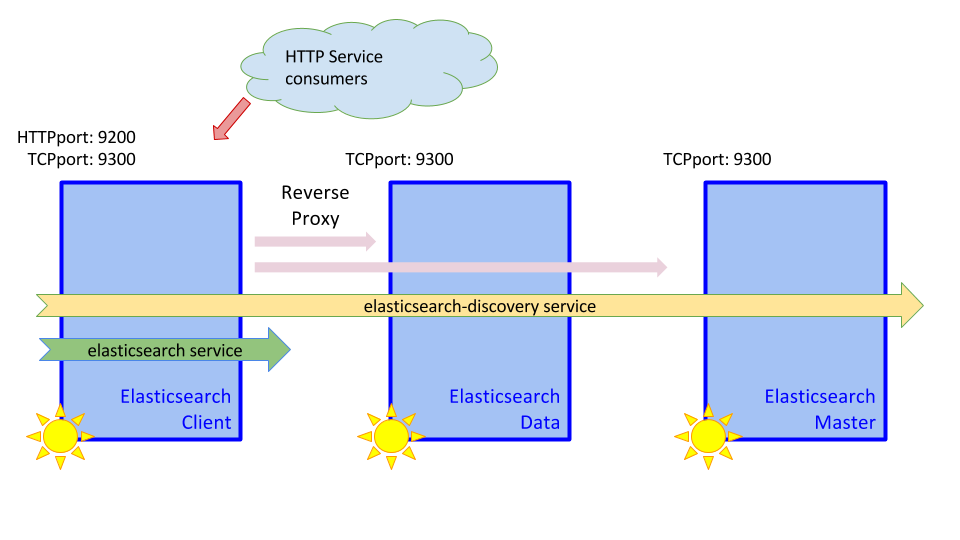
\includegraphics[height=6cm]{fe-consumers}
		\caption{Architettura del \textit{backend} applicativo.}
	\end{center}
\end{figure}

Il traffico tra i processi Elasticsearch è di due tipi. Il primo traffico 
riguarda quello di servizio ed interno del cluster, è un traffico non visibile 
dall'esterno ed è necessario per coordinare i singoli nodi del cluster, il protocollo 
utilizzato è HTTP e la porta logica è 9300. Sempre attraverso il protocollo HTTP e porta 9200
ho esposto il servizio di Elasticsearch ad ogni altro microservizio consumatore. 
Il traffico entrante è diretto verso il nodo client che in modalità \textit{reverse proxy}
inoltra le richieste ai membri del cluster. Il traffico tra le componenti del 
cluster Elasticsearch è criptato tramite un token. Ogni componente del sistema 
è associata con un utente che ha determinati privilegi. In figura, ho rappresentato 
il token di sicurezza tramite un sole di color giallo. 

L'utente interagisce con il microservizio di gestione delle dashboard.
La tecnologia utilizzata è un applicazione web, che nativamente è 
pensata per comunicare con Elasticsearch. Quest'applicazione, 
essendo priva di stato, è facilmente scalabile in orizzontale.

\begin{figure}[htbp]
	\begin{center}
		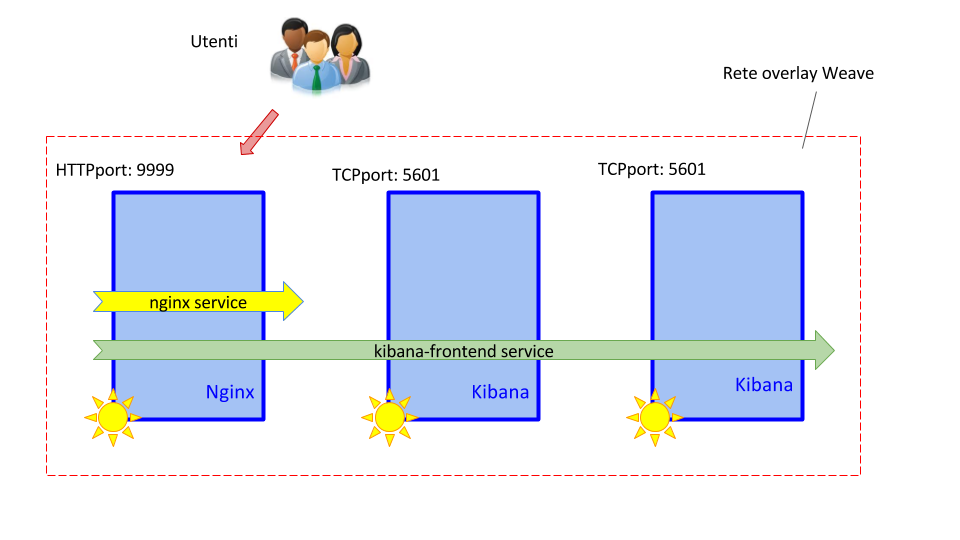
\includegraphics[height=6cm]{elk-cluster}
		\caption{Architettura del \textit{frontend} applicativo.}
	\end{center}
\end{figure}

Il sistema espone un unico punto di accesso alle dashboard. 
Ogni utente per accedere al sistema deve essere registrato.
Solo dopo un'autenticazione l'utente può utilizzare il servizio.
Inoltre, per garantire che solo determinati utenti possano accedere al
servizio, il sistema effettua un filtraggio base sugli indirizzi IP.
Infatti, solo gli indirizzi IP nella lista bianca vengono accettati
dal sistema. In caso di altri indirizzi IP, il sistema ignora le richieste.  

Per l'implementazione del microservizio di autenticazione ed autorizzazione 
ho utilizzato Nginx. Nginx è un \textit{load balancer} a livello L7 (Layer 7 OSI), 
bilanciatore del traffico a livello HTTP.

Un'ulteriore questione che ho trattato è il dimensionamento delle componenti 
del sistema. 

\begin{figure}[htbp]
	\begin{center}
		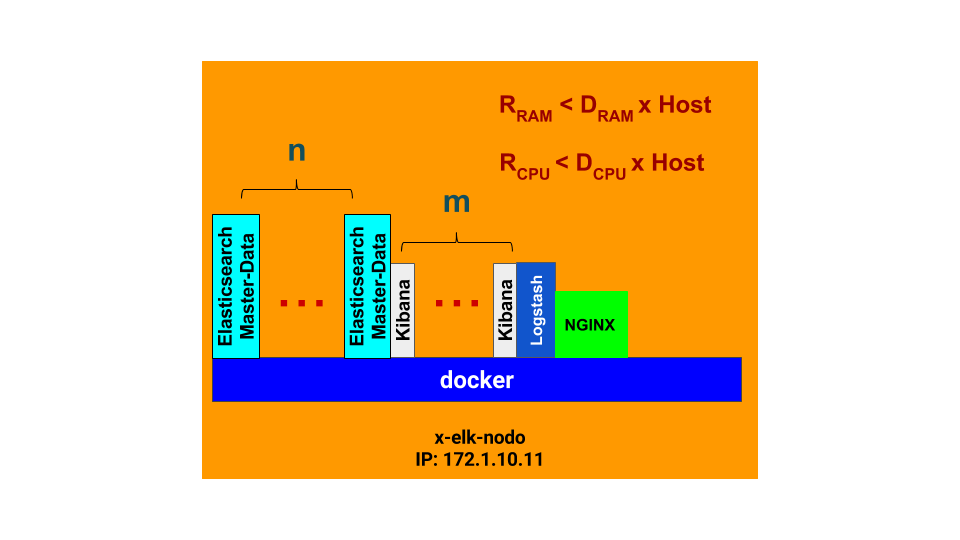
\includegraphics[height=6cm]{dimensionamento}
		\caption{Visione d'insieme per macchina virtuale della richiesta di risorse fisiche.}
	\end{center}
\end{figure}

Ciascuna componente specifica una quantità fissa di risorse. 
Questa quantità non è statica e può variare nel tempo. Durante le 
valutazioni di dimensionamento ho cercato di garantire che il 
totale delle risorse richieste da un insieme di componenti, in una specifica
macchina virtuale, non superi la quantità fisicamente disponibile.
In caso di sovrastima, le macchine virtuali subiranno il OOM (Out of memory).

\newpage   

\subsection{Lo \textit{Storage}}

In contesto containerizzato con orchestratore,
ho utilizzato le risorse di Kubernetes per
isolare le dipendenze delle componenti applicative verso 
il server fisico che gestisce la memorizzazione dei
dati e la loro disponibilità inter macchine virtuali. 

Come \textit{tool} per la condivisone fisica dei dati 
tra le macchine virtuali ho utilizzato il NFS (Networked File System).
Ho valutato anche la tecnologia GlusterFS di RedHat. In seguito a una 
sessione di \textit{brainstorming} con il mio tutor 
abbiamo deciso che la tecnologia per lo \textins{storage distribuito} 
è molto valida e adatta per i container., tuttavia, aggiunge
complessità al progetto. Come conseguenza di questa sessione, 
io e il mio tutor abbiamo confermato l'utilizzo della tecnologia 
NFS.
  
\begin{figure}[htbp]
	\begin{center}
		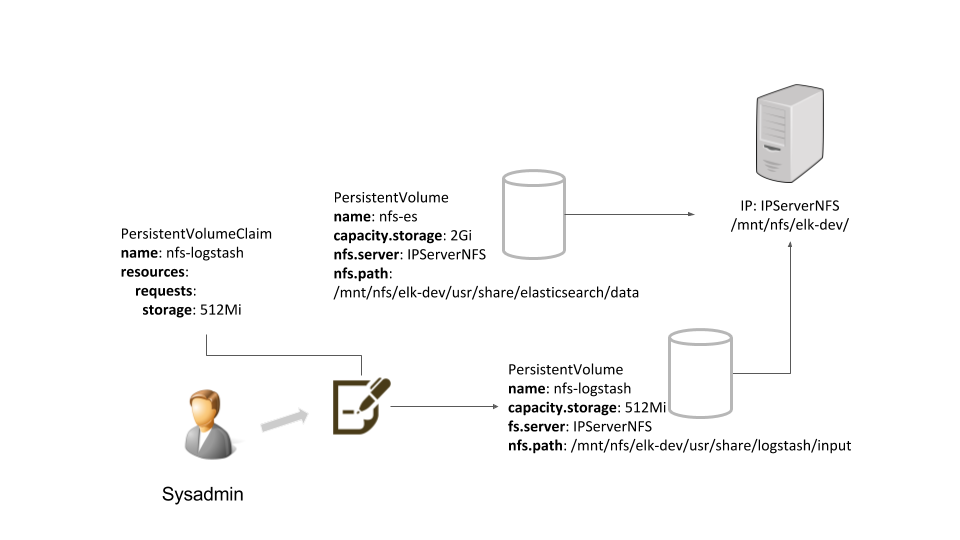
\includegraphics[height=7cm]{storage}
		\caption{Organizzazione logica dei dati e i livelli di astrazione degli accessi ai dati.}
	\end{center}
\end{figure}

Kubernetes ha il compito di orchestrare i container. Molto spesso, 
Kubernetes schedula un container su una VM e in seguito, in caso 
di non disponibilità di risorse fisiche (CPU, RAM), 
lo scheduler della piattaforma schedula l'esecuzione del 
container su un'altra macchina virtuale. Questo fenomeno 
è comunemente chiamato migrazione.  Il modo con cui Docker e Kubernetes 
esportano i dati dal container sono i volumi. Tuttavia, i volumi 
introducono una dipendenza forte con il host che ospita il container 
in esecuzione. Inoltre, i volumi creati su un host non sono
visibili e raggiungibili da qualunque altro host nella rete.

Kubernetes, tramite gli oggetti per la gestione dei volumi, elimina
l'accoppiamento dei container con l'ambiente virtuale specifico
di esecuzione.

In figura presento i livelli di astrazione usati da Kubernetes 
per garantire la visibilità dei dati tra VM durante la migrazione dei container.
Gli oggetti per la gestione dei dati sono i PersistentVolume e
PersistentVolumeClaims. 

Con i PersistentVolume definisco una capacità di dati che può essere fisicamente 
allocata sul disco fisico di una macchina virtuale. E questa capacità 
è utilizzabile globalmente da tutti i microservizi che hanno accesso. 
Invece, con i PersistentVolumeClaim definisco un sottoinsieme della 
capacità specificata dai PersistentVolume. 
Questo modo di gestire i dati mi permette di rendere indipendente la 
modalità di memorizzazione dei dati su disco dalla modalità di consumo 
dei dati da parte delle componenti containerizzate.
Una simile razionalizzazione dello storage mi offre la possibilità
di portare i dati in qualsiasi ambiente, da un volume NFS a un volume sul
cloud di Amazon oppure Azure ed ecc.

Con l'orchestratore la gestione dei dati è semplice.
In assenza dell'orchestratore la complessità  
è proporzionale al numero dei container da gestire.
Per l'ambiente senza orchestratore ho utilizzato ampiamente
il pattern sidecar applicato allo storage.
La  rappresentazione del pattern segue in figura.   

\begin{figure}[htbp]
	\begin{center}
		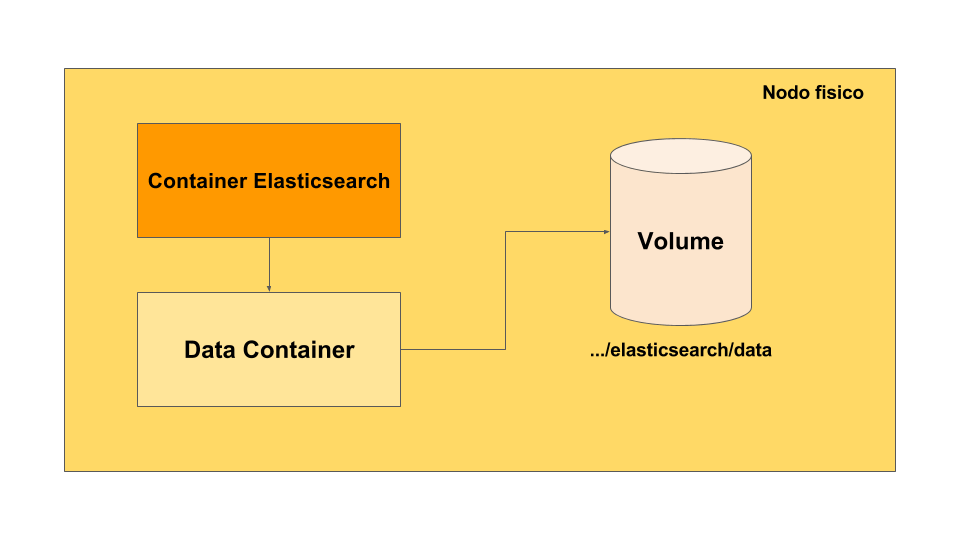
\includegraphics[height=6cm]{data-container}
		\caption{Riduzione della dipendenza dei dati dall'infrastruttura fisica in contesto senza orchestratore.}
	\end{center}
\end{figure}

Un alias del sidecar pattern è il \textit{data container}. 
Ho utilizzato questo pattern per progettare la 
l'accesso di scrittura e lettura dei dati a livello
globale senza la necessità di specifica di indirizzi IP. 
Infatti, i container applicativi del sistema 
per accedere ai dati semplicemente 
utilizzano il nome del data container. Dal punto 
di vista dei pattern di progettazione di dettaglio,
un data container è un pattern Singleton. 

%\newpage

\subsection{Il \textit{Networking}}

La rete è un altro aspetto importante nel 
contesto della \textit{light virtualization}.
Kubernetes richiede come vincolo che ad ogni 
Pod venga assegnato un indirizzo IP univoco. 
La necessità di utilizzare un indirizzo IP univoco per 
container è necessaria per evitare la complessità di gestione 
delle porte logiche su cui esporre i servizi.
Inoltre, Kubernetes gestisce il traffico 
tra container tramite regole di routing di basso livello
e gestito in modo automatico. Il traffico del cluster Kubernetes 
è gestito dalla componente Kube-Proxy.
Per assegnare indirizzi univoci ai Pod, ho utilizzato
il plugin WeaveNet. 
Questo strumento mi ha permesso di creare una 
rete \textit{full mesh} tra i container.

\begin{figure}[htbp]
	\begin{center}
		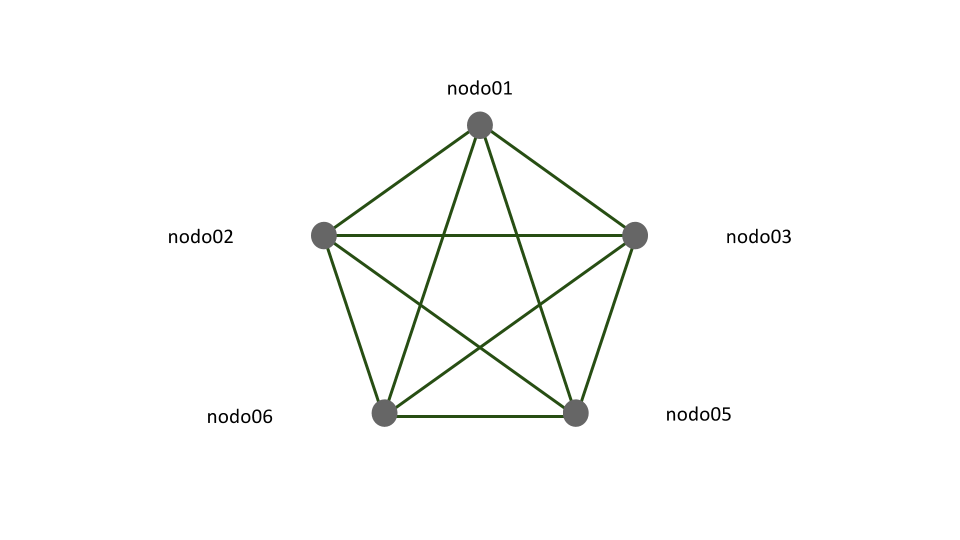
\includegraphics[height=6cm]{networking}
		\caption{Visione di alto livello della topologia di rete.}
	\end{center}
\end{figure}

WeaveNet crea una rete virtuale distribuita su tutte le macchine 
virtuali. L'obbiettivo principale dello strumento è l'assegnazione 
degli indirizzi IP alle risorse Kubernetes \textit{on-demand}. 
La classe degli indirizzi allocabili dalla componente WeaveNet è di tipo A 
(10.1.0.0/16).  
Il prodotto WeaveNet è caratterizzato da un insieme di agenti che cooperano
per gestire il routing del traffico di rete nel modo più ottimale possibile.
Ho gestito il deployment degli agenti WeaveNet tramite l'utilizzo 
della risorsa DeamonSet. Questa risorsa è una estensione della risorsa
Deployment. Tramite la risorsa del DaemonSet, in caso di aggiunta di nodi al 
cluster Kubernetes, il controller del cluster schedulerà dinamicamente 
una istanziazione dell'agente sul nuovo nodo
senza alcun intervento manuale.

Ho utilizzato la ridondanza a livello della rete virtuale per incrementare 
l'alta affidabilità della rete stessa. Infatti, in caso di un problema con 
qualche agente WeaveNet, i pod possono continuare a comunicare con le 
altre componenti in modo trasparente. 

%\newpage

\section{Test}
I test che ho effettuato durante lo stage, per la 
verifica del sistema, sono i test di carico e i test di durata. 
Ho valutato diversi strumenti open source idonei per questa 
tipologia di test. Lo strumento che ho scelto per effettuare i test è JMeter.
La peculiarità di JMeter, che mi ha impressionato, è il variegato 
insieme di plugin e l'insieme di configurazioni che esso supporta.

\begin{center}
	\begin{tabular}
		{l||p{5cm}}	
		\arrayrulecolor{white}
		\rowcolor{glaucous}	
		Configurazione VM & 
		\makebox[5cm][c]{Valore}\\
		\rowcolor{lightcornflowerblue}
		Sistema Operativo &
		\makebox[5cm][c]{CentOS7}\\
		\rowcolor{moonstoneblue}
		Kernel &
		\makebox[5cm][c]{3.10.x86-64}\\
		\rowcolor{lightcornflowerblue}
		CPU(s) &
		\makebox[5cm][c]{4} \\
		\rowcolor{moonstoneblue}
		RAM &
		\makebox[5cm][c]{4GB}\\ 
		\rowcolor{lightcornflowerblue}
	\end{tabular}		  
\end{center}
\captionof{table}{Parametri di configurazione comuni delle macchiane vituali utilizzate durante i test.}

Il taglio di macchine virtuali che ho utilizzato è medio-piccola.
Ho scelto una simile configurazione perché è una categoria molto frequente in cloud.
Questo taglio di macchine sono caratterizzate da un prezzo conveniente. Effettuare 
i test su questo taglio di macchine permette di paragonare i test fatti da altri
con i risultati da me ottenuti.

\subsection{Obiettivi dei test}
Analizzare, progettare ed implementare i test è un forma d'arte.
L'obiettivo principale dei test è lo studio del comportamento
del sistema nel complesso e nell'ambiente containerizzato 
con orchestratore Kubernetes. Per effettuare i test ho fissato 
i limiti di memoria e CPU per ciascuna componente containerizzata. 

Gli obiettivi che ho individuato per i test sono i seguenti:

\begin{itemize}
	\item Studiare il comportamento di Elasticsearch a regime e 
	      sotto carico di lavoro con le configurazioni da me individuate;      
	\item Individuare il punto di rottura del sistema, oltre al quale  
	      il livello di servizio degrada;
	\item Confrontare, a pari di configurazione, il sistema containerizzato 
		  con un sistema containerizzato.
\end{itemize}

\subsection{Metodologia}

In seguito alla preparazione dell'ambiente di test, 
ho individuato degli scenari possibili di test. 
Tramite uno scenario cerco di simulare l'attività 
dell'utente con il sistema. L'utente virtuale deve 
effettuare una serie di richieste di complessità sempre
crescente. Le richieste riguardano la visualizzazione 
delle dashboard. Durante le prime visualizzazioni
l'utente virtuale visualizza i singoli elementi 
alla base di una dashboard complessa. E successivamente 
tramite aggregazione l'utente effettua visualizzazioni
sempre più complesse e numerose.
Con JMeter ho codificato degli script per i scenari di test. 
Un esempio di script, che allego in figura per il test di durata, 
ha lo scopo di simulare 100 utenti che interagiscono con il sistema 
in un intervallo temporale di un'ora. 

\begin{figure}[htbp]
	\begin{center}
		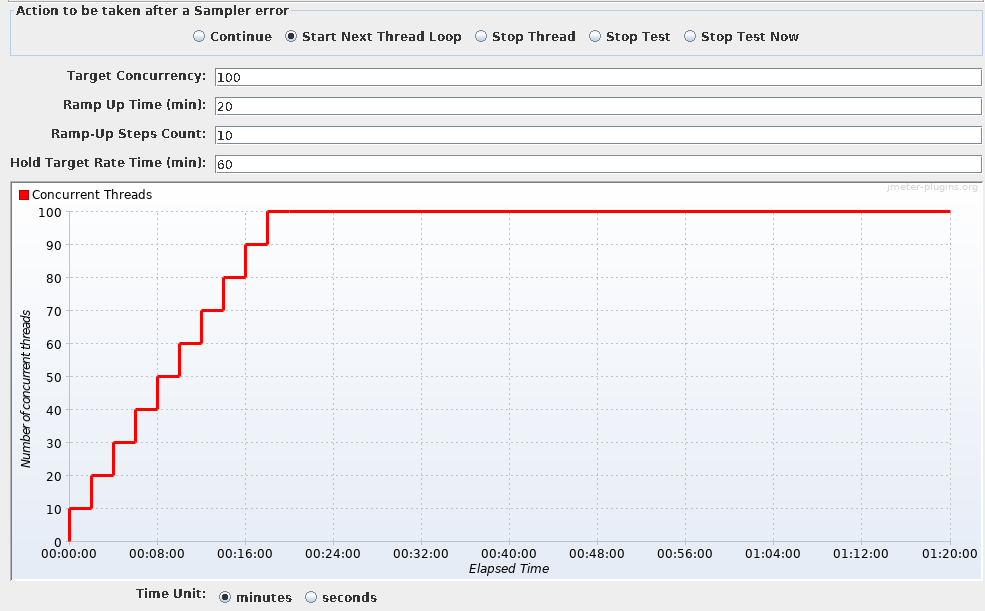
\includegraphics[height=6cm]{jmeter}
		\caption{Script JMeter per i test di durata con 100 utenti, 1h di durata.}
	\end{center}
\end{figure} 

La configurazione utilizzata per lo scenario del test 
è come nella tabella seguente.

\begin{center}
	\begin{tabular}
		{l||p{5cm}}	
		\arrayrulecolor{white}
		\rowcolor{glaucous}	
		Parametro di configurazione &  
		\makebox[5cm][c]{Valore} \\
		\rowcolor{lightcornflowerblue}
		Utenti & 
		\makebox[5cm][c]{100} \\
		\rowcolor{moonstoneblue}
		Tempo d'inizializzazione & 
		\makebox[5cm][c]{20 minuti} \\
		\rowcolor{lightcornflowerblue}
		Fasi di inizializzazione & 
		\makebox[5cm][c]{10}  \\
		\rowcolor{moonstoneblue}
		Durata test & 
		\makebox[5cm][c]{60 minuti}\\ 
		\rowcolor{lightcornflowerblue}
	\end{tabular}		  
\end{center}
\captionof{table}{Paramentri di configurazione di uno scenario di esempio del test di durata.}

Come output, per ciascun test in parte ho generato un resoconto finale.
Per la creazione dei report, ho progettato ed implementato un processo automatico.
Ho scelto le ore notturne per effettuare i test e generare i report per i seguenti
motivi: 
\begin{itemize}
	\item Utilizzare le ore di lavoro regolari per fare analisi e studio dei dati;
	\item Impiegare i server fisici di IKS al massimo durante le ore notturne;
	\item Ridurre al minimo gli impatti delle eventuali interferenze sulle macchine 
	      virtuali da me utilizzate.  
\end{itemize}


\subsection{Risultati}
Durante i test, ho appreso che con specifiche configurazioni di memoria, CPU e 
topologia del cluster Elasticsearch il sistema è più responsivo. 
Ottenere una configurazione del sistema con specifici limiti sulle
non è stato facile. Questa ricerca ha rafforzato la mia confidenza 
con l'amministrazione del cluster Kubernetes.
 
In figura a seguire, presento il comportamento dei tempi di risposta in 
relazione con il numero di utenti attivi nel sistema. 

\begin{figure}[htbp]
	\begin{center}
		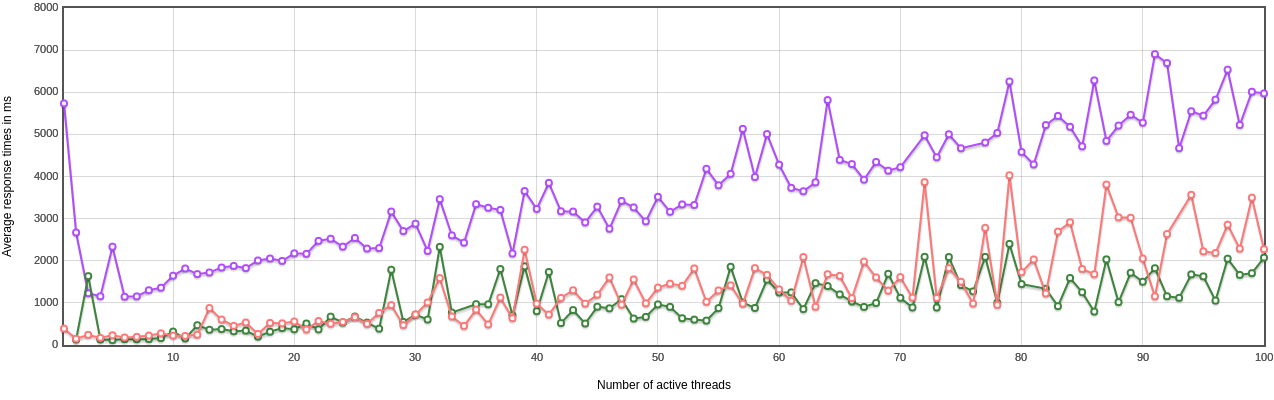
\includegraphics[height=5cm]{flotTimesVsThreads}
		\caption{Andamento dei tempi di risposta all'aumentare del numero degli utenti.}
	\end{center}
\end{figure}

Qui, il numero dei thread rappresentano il numero di utenti attivi nel sistema. 
I dati mostrano che all'aumentare del numero degli utenti, per le tre 
attività di visualizzazione di dashboard, i tempi di risposta sono 
sempre al di sotto dei 9 secondi. Questo è un buon risultato, assumendo 
come limiti di attesa i 10 secondi per ottenere la visualizzazione di una 
pagina, durante l'attività di carico del sistema. Ho recuperato
questa immagine da uno dei report che il processo di test ha generato.

\newpage
\section{Monitoraggio}

Il monitoraggio delle applicazioni e dell'infrastruttura 
è un aspetto molto importante. Sia Docker sia Kubernetes 
non offrono soluzioni native di monitoraggio. I comuni 
strumenti di monitoraggio, orientati a macchine virtuali, 
non sono più idonei. Le macchine virtuali hanno un tempo di
accensione di un ordine di grandezza superiore rispetto 
ai container. Se le macchine virtuali operano nell'ordine 
dei minuti, allora i container operano nell'arco dei secondi. 

Visto che non esiste una soluzione nativa per l'esportazione delle
metriche in Docker, ho utilizzato la componente cAdvisor che
esporta i dettagli da monitorare nel comodissimo formatto JSON. 
Definito il modo per l'estrapolazione delle informazioni 
sui container, ho integrato cAdvisor con InfluxDB, un \textit{timeseries database}, 
e Graphana, una componente di visualizzazione. Quest'ultima offre 
un familiare DSL (\textit{Domain Specific Language}) 
in stile SQL (\textit{Search Query Language}).  

Un'ulteriore componente che ho utilizzato per il monitoraggio 
dell'infrastruttura è la \textit{dashboard} di Kubernetes.
Oltre al monitoraggio, la dashboard nativa di Kubernetes
offre la possibilità di scrivere nuovi manifest, editare 
e cancellare quelli esistenti. Oltre alla creazione di risorse
è possibile visionare i log per ciascun container da un unico 
punto di accesso. La dashboard centralizza la gestione del cluster. 

In conclusione di stage, mi sono reso conto che la visione 
d'insieme del cluster e del sistema realizzato è poco chiara. 
Uno svantaggio di un sistema containerizzato è la mancanza 
della rappresentazione grafica delle relazioni tra le componenti.
Questo è dovuto alla natura distribuita dei microservizi. 
Con questo fatto in mente, ho ridotto la difficoltà di gestione
tramite uno strumento open source. Il nome di questo strumento 
è Weave Scope. 

\begin{figure}[htbp]
	\begin{center}
		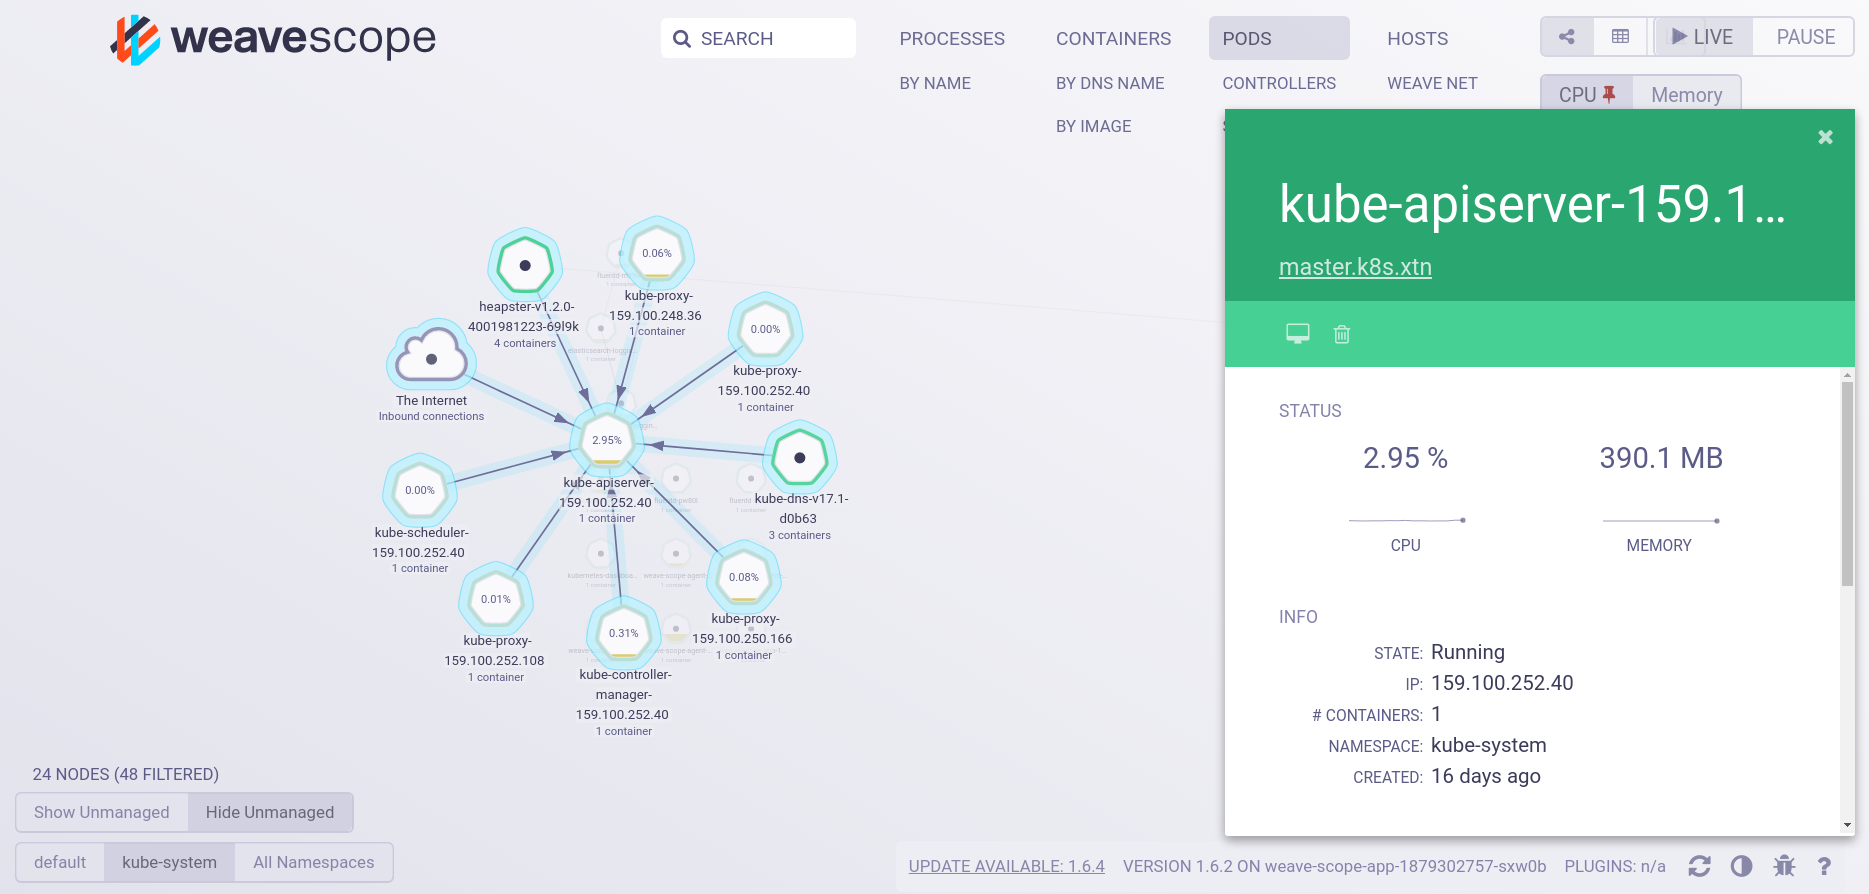
\includegraphics[height=7.5cm]{pods}
		\caption{Grafo dei Pod a supporto del cluster Kubernetes.}
	\end{center}
\end{figure} 
\newpage
Per lo studio del consumo delle risorse, il prodotto di Weaveworks
offre una vista dello stato delle risorse sul server. In figura 
illustro qual è lo stato delle risorse del nodo master del cluster K8s.
\begin{figure}[htbp]
	\begin{center}
		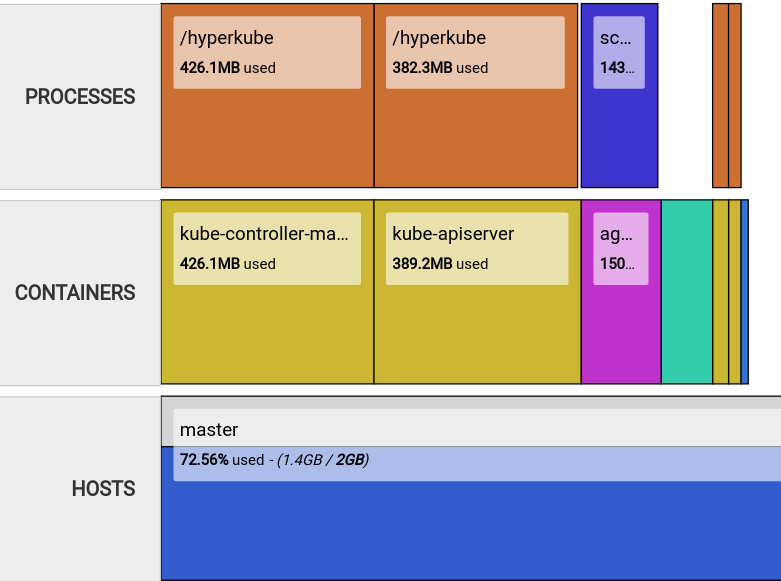
\includegraphics[height=5cm]{resource-consumption}
		\caption{Vista del consumo di risorse su un nodo del cluster Kubernetes.}
	\end{center}
\end{figure}

In conclusione, illustro la visione completa del sistema 
dal punto di vista delle componenti. Ogni componente 
è presentata in versione ridondata.
\newpage
\begin{figure}[htbp]
	\begin{center}
		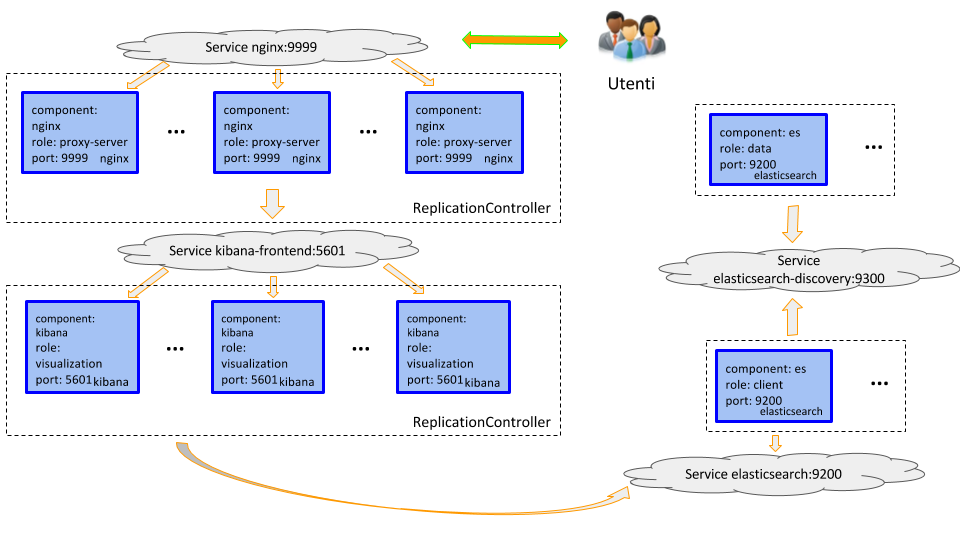
\includegraphics[height=7cm]{panoramica-sistema}
		\caption{Visione completa delle componenti del sistema e delle loro relazioni.}
	\end{center}
\end{figure}
\newpage
